\apendice{Especificación de Requisitos}

\section{Introducción}
En este apéndice se detallan los requisitos del proyecto, como los funcionales y no funcionales. La finalidad es hacer de intermediario entre el cliente y los programadores, con el objetivo de ayudar a entender, comprender y analizar la aplicación. 

\section{Objetivos generales}
Este trabajo final de grado focaliza la aplicación mediante dos puntos de vista totalmente diferentes, dependiendo de las situaciones futuras a las que se someta la aplicación, siempre englobado en el marco de que es un producto que nos encarga la universidad de Burgos, como cliente final.

\begin{itemize}
	\item Colección de videojuegos. Tener una gran cantidad de estos mismos, para lograr sacar un rendimiento económico gracias a lo publicidad, por lo que es necesario que la aplicación tenga una gran repercusión en el mercado. Esto implica que a futuro se debe de hacer una inversión en publicidad y \emph{marketing}.
	\item \emph{Porfolio} \cite{wiki:portafolio} o escaparate con el que mostrar las capacidades técnicas, herramientas usadas o lenguajes de programación aprendidos, ante los equipos de recursos humanos en las empresas, llegado el momento de tener que buscar trabajo. 
\end{itemize}

\section{Catalogo de requisitos}
A continuación se numeran los requisitos del proyecto extraídos de los generales.

\subsection{Requisitos funcionles}
Por cada uno de los requisitos funcionales, va a tener una correlación con la pantalla en la que se da la operatividad del mismo, excepto en los casos en las que este requerimiento abarca varias ventanas.

Algunos de los requisitos funcionales, en el momento de ser tratados con el cliente, tuvieron apoyo de unos \emph{sketch} o bocetos conceptuales, con el fin de dar soporte, ayudar a comprender y facilitar la comunicación cliente - analista. Como podemos ver en la imagen~\ref{fig:bocetolog}, o en el apéndice de diseño~\pageref{diseño}.

\begin{figure}[H]
	\centering
	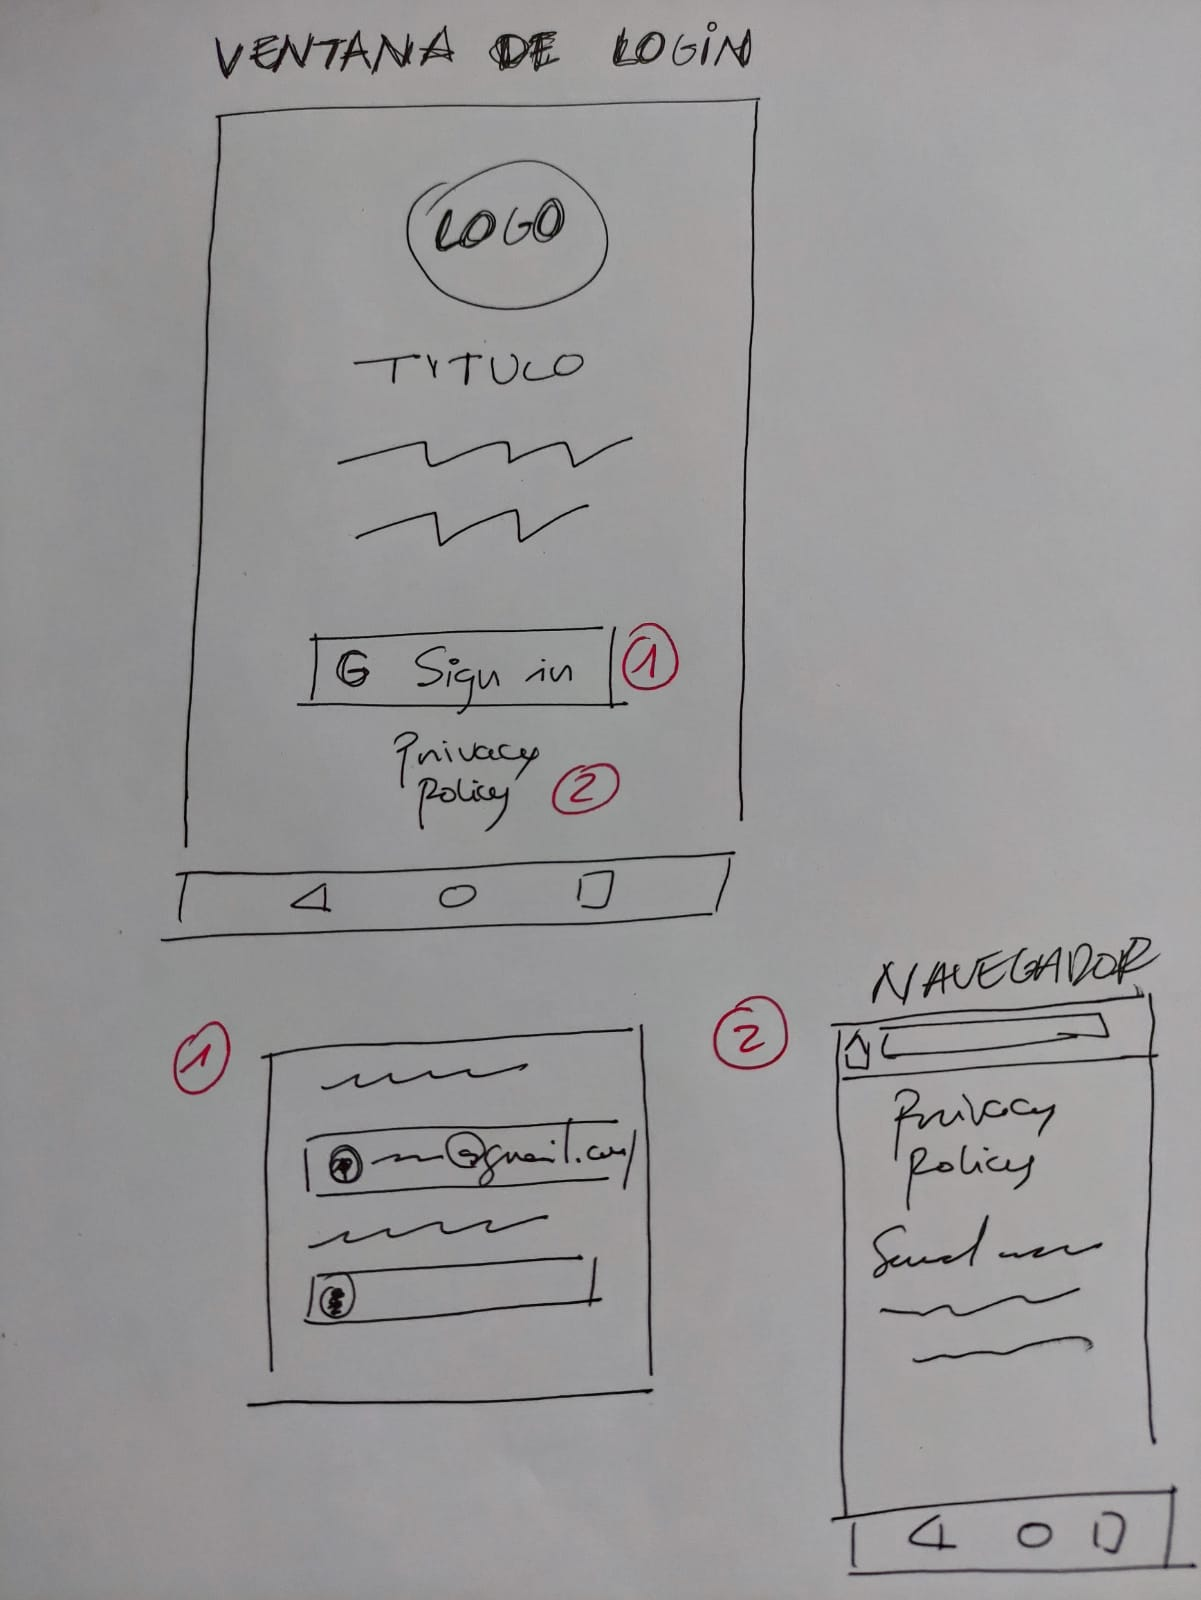
\includegraphics[height=0.9\textwidth]{requisitos/bocetolog.jpeg}
	\caption{Boceto sing in}\label{fig:bocetolog}
\end{figure}

\begin{itemize}
\tightlist
	%%INICIO DE LA SESIÓN
	\item \textbf{RF-1 Ventana de \emph{sign in:}~\ref{fig:loginpage}} La aplicación tiene que contener una ventana principal con la que los usuarios puedan iniciar la sesión, con el fin de tener servicios en la nube.
	
	\begin{itemize}
	\tightlist
	\item \textbf{RF-1.1 Botón de inicio sesión:} Mediante un elemento clickable se debe de tener acceso a un formulario para poder entrar mediante la cuenta de \emph{Google}.
	\item \textbf{RF-1.2 Consultar la política de privacidad:} Un enlace en el que se pueda mostrar todo lo referente a la política de privacidad.
	\item \textbf{RF-1.3 Cerrar sesión:} ser capaz de salir de la aplicación \emph{sign out}, desde cualquier ventana.
	\end{itemize}
	
	%% MENÚ DE NAVEGACIÓN PERMANENTE DURANTE LA EJECUCIÓN
	\item \textbf{RF-2 Menú de navegación:~\ref{fig:menuhome}} Se considera necesario tener la capacidad de navegar de una parte a otra dentro de la aplicación, sin tener que pasar entre ventanas, mediante un menú. 
	
	\begin{itemize}
		\tightlist
		\item \textbf{RF-2.1 Menú lateral} el usuario debe poder entrar al menú mediante un \emph{scroll lateral}.
		\item \textbf{RF-2.1 Integración con el RF-1.3:} Para que se disponga la salida en cualquier momento de la aplicación es necesario incluir en el menú, los datos de usuario con la capacidad de salir.
	\end{itemize}

	%% ALGUNOS DE LOS AJUSTES DEBEN DE SER SELECCIONABLES
	\item \textbf{RF-3 Ventana de opciones~\ref{fig:settingspage}} la aplicación tiene que ser capad de gestionar algunas de las diferentes capacidades del producto, que el usuario desee.
	
	\begin{itemize}
		\tightlist
		\item \textbf{RF-3.1 Opción \emph{dark mode}:} la aplicación tiene que ser capada de cambiar el color del sistema, para ahorrar batería o para mejorar el contraste.
		\item \textbf{RF-3.2 Opciónes del juego snake:} algunas de las opciones de este juego deben de ser controlables desde el apartado de ajustes.
	\end{itemize}
	
	%% INFORMACIÓN RELEVANTE SOBRE EL CREADOR DE LA APLICACIÓN
	\item \textbf{RF-4 Ventana de \emph{about}~\ref{fig:aboutpage}} mostrar información sobre el creador de la aplicación.
	
	\begin{itemize}
		\tightlist
		\item \textbf{RF-4.1 Opción \emph{dark mode}:} la aplicación tiene que ser capada de cambiar el color del sistema, para ahorrar batería o para mejorar el contraste.
		\item \textbf{RF-4.2 Opciónes del juego snake:} algunas de las opciones de este juego deben de ser controlables desde el apartado de ajustes.
	\end{itemize}
	
	%% PUBLICIDAD INTEGRADA
	\item \textbf{RF-5 Publicidad integrada} la aplicación debe de ser capad de mostrar anuncios.
	
	\begin{itemize}
		\tightlist
		\item \textbf{RF-5.1 Publicidad mediante \emph{banner}:} mostrar en el \emph{footer} un contenedor de anuncios, proporcionados estos por Google.
		\item \textbf{RF-5.2 Continuar Snake:} el usuario tiene que ser capad de ver un video, como recompensa, continuar en la partida. 
	\end{itemize}

	%% JUEGO DEL SNAKE
	\item \textbf{RF-6 Juego del snake \ref{fig:snakepage}:} el usuario tiene que ser capad de jugar a este juego.
	
	\begin{itemize}
		\tightlist
		\item \textbf{RF-6.1 Control juego:} la aplicación tiene que ser capad de trabajar con los choques que se producen, con la comida, pared, bloques, o tuberías.
		\item \textbf{RF-6.2 Mostrar la puntuación:} la aplicación tiene que ser capad de mostrar la puntuación que lleva en la partida.
		\item \textbf{RF-6.3 Compartir la puntuación:} el jugador tiene que ser capad de subir la puntuación una vez termine la partida. Siempre y cuando esta sea mejor a otra anterior.
		\item \textbf{RF-6.4 Mostrar el ranking:} el usuario tiene que ser capad de ver la puntuación del resto de jugadores, así como la que ha logrado.
	\end{itemize}

	%% JUEGO DEL CUATRO EN RAYA
	\item \textbf{RF-7 Juego del cuatro en raya \ref{fig:cuatromenu}:} el usuario tiene que ser capad de jugar a este juego.
	
	\begin{itemize}
		\tightlist
		\item \textbf{RF-7.1 Invitar:} el usuario tiene que ser capad de invitar a otro jugador, compartiendo una clave de acceso a la partida. Tiene que haber un botón que ayude a hacer esta tarea.
		\item \textbf{RF-7.2 Unirse:} el usuario mediante un formulario debe de ser capad de ingresar la clave de acceso de la parida.
		\item \textbf{RF-7.3 Dinámica del juego:} la aplicación tiene que ser capad de controlar los diferentes eventos se producen durante la partida, como pueden ser, sorteo de inicio, ficha no válida, formación del cuatro en raya, advertir de quien gana.
		\item \textbf{RF-7.4 Hablar mediante chat:} el usuario tiene que ser capad de mandar mensajes cortos, de no más de 15 caracteres. Después de remitir el mensaje, se tiene que bloquear esta opción durante 10 segundos, para no sobrescribir otros mensajes o que se sature el juego.
	\end{itemize}

\end{itemize}


\section{Especificación de requisitos}


